\documentclass[10pt,a4paper,twocolumn]{article}
\usepackage[margin=19mm,columnsep=7mm]{geometry}
\usepackage{amsmath,amssymb,amsthm,graphicx,booktabs,hyperref}
\usepackage[T1]{fontenc}
\hypersetup{hidelinks}
\newtheorem{theorem}{Theorem}
\newtheorem{proposition}{Proposition}
\newcommand{\R}{\mathbb R}
\newcommand{\Z}{\mathbb Z}
\newcommand{\N}{\mathbb N}
\newcommand{\sgn}{\operatorname{sgn}}
\newcommand{\tr}{\operatorname{tr}}
\newcommand{\conv}{\operatorname{conv}}
\title{Recursive Triforce Closure of the Dual Tetrad:\\Dyadic Depth, Channel Parity and the Connection Dictionary}
\author{Field Dynamics Research}
\date{26 November 2026\\\small Mathematical manuscript; Lean build pending}
\begin{document}
\maketitle
\begin{abstract}
The complementary tetrahedra of the forced spatial tetrad distinguish a central triangular region and three lateral regions on each face. We show that their full medial refinement, on the additive lattice generated by the central octahedron's edge midpoints, has maximal complete dyadic depth two. The entire lattice intersection of a face is the fifteen-point quarter barycentric grid, whose elementary nearest-neighbour mesh has sixteen triangles. Pairing inverted faces gives sixty-four geometric addresses with pointing multiplicities forty and twenty-four. We construct a graded isomorphism to the symmetric and antisymmetric connection-slot spaces under proper tetrahedral permutations, prove the obstruction under the full reflection-inclusive group, and give an explicit signed repair of its action. A reversible four-way tree has twenty-one internal readers and a distinct twenty-one-dimensional invariant contrast space. These are geometric and representation-theoretic results. The physical selection of the lattice, independent field amplitudes, dynamical connection and gravitational source operator are not assumed or established. An independent exact verifier passes 214 checks; the accompanying Lean source has not yet been kernel-compiled.
\end{abstract}

\section*{Setting}
Let $I=\{0,1,2,3\}$, and let $s_i$ be the sign vectors $(1,1,1),(1,-1,-1),(-1,1,-1),(-1,-1,1)$. We use the two solids $\conv(S)$ and $\conv(-S)$, where $S=\{s_i:i\in I\}$. The half-space proof identifies their overlap as $\conv(\pm e_1,\pm e_2,\pm e_3)$, the regular octahedron. We name a face by its omitted vertex $i$, pairing it with the inverted face in the other solid. This is an address quotient, not an identification of the two chambers' values. The half-space proof uses the opposite chamber naming convention to the sign-vertex convention here; the statements are independent of the name.\footnote{The upstream formalization calls $\conv(S)$ TetB. The inherited Lean hull theorem uses that convention.}

\section*{The medial refinement}
\begin{theorem}
On a nondegenerate triangular face, the central similarity $F_i(x)=c-(x-c)/2$, with centroid $c$, and the three corner similarities $F_j(x)=(x+v_j)/2$ partition the face into four equal-area triangles with disjoint relative interiors. The depth-$n$ refinement consists of $4^n$ triangles with $(2^n+1)(2^n+2)/2$ distinct vertices.
\end{theorem}
\begin{proof}
In barycentric coordinates $\lambda_1+\lambda_2+\lambda_3=1$, $\lambda_j\ge0$, the corner map at $j$ sends $\lambda$ to $(\lambda+e_j)/2$. Its inverse on the region $\lambda_j\ge1/2$ is $2\lambda-e_j$. The central map sends $\lambda$ to $(\mathbf1-\lambda)/2$, whose inverse is $\mathbf1-2\lambda$ on the region where all coordinates are at most $1/2$. These regions cover the simplex and their interiors cannot overlap: two coordinates cannot both exceed one half. Each affine map scales lengths by one half and areas by one quarter. In two dimensions the determinant of $-I/2$ is positive, so reversing pointing does not reverse planar orientation.

Iterating the maps tiles each child in the same manner. At depth $n$ the sides have $2^n$ equal steps, and the vertices are the barycentric triples with nonnegative integer numerators of sum $2^n$. The elementary triangular rows of this grid are obtained by the same subdivision, by induction on $n$. Their number of vertices is $\binom{2^n+2}{2}$. Boundaries have shared edges and vertices, not shared relative interiors.
\end{proof}
The first central region is the intersection of the face with the complementary chamber: for a face of $\conv(S)$, the barycentric expression gives $s_j\cdot x=4\lambda_j-1$ for $j\ne i$, and $s_i\cdot x=-1$. Membership of the opposite tetrahedron requires $s_j\cdot x\le1$, precisely $\lambda_j\le1/2$. The subsequent subdivision is mathematical; no dynamics has been used.

\section*{The midpoint lattice and its full mesh}
\begin{theorem}
Let $L$ be the additive group generated by the twelve central-octahedron edge midpoints. Then
\begin{equation}
 L=\tfrac12\{z\in\Z^3:\textstyle\sum z_j\equiv0\pmod2\}.
\end{equation}
Projection along a face normal gives the triangular Flower lattice. Complete dyadic refinement has all vertices in $L$ if and only if $n\le2$. On each face the full lattice intersection is the depth-two grid, with fifteen vertices, thirty primitive nearest-neighbour edges and sixteen elementary triangles.
\end{theorem}
\begin{proof}
The doubled edge midpoints are the signed permutations of $(1,1,0)$. All have even sum. Conversely the three positive generators $(1,1,0),(1,0,1),(0,1,1)$ span every even-sum integer triple $(x,y,z)$, since their coefficients are $(x+y-z)/2,(x+z-y)/2,(y+z-x)/2$. Their integrality is equivalent to even total sum.

For the reference normal $s_0$, write $P=I-\mathbf1\mathbf1^T/3$. In the basis $p=P(e_1)/2$, $q=P(e_2)/2$, a projected doubled lattice point $(x,y,z)$ has coordinates $(x-z,y-z)$. Every such pair is integral, and the projected negative edge midpoints $(-e_2-e_3)/2$, $(-e_1-e_3)/2$ give $p,q$. Thus $P(L)=\Z p+\Z q$. The tetrahedral symmetries transport this to each face's own normal plane.

Every vertex belongs to $L$ and every edge displacement is a signed permutation of $(0,2,2)$. At depth $n$ the first edge step has doubled nonzero coordinate $4/2^n$, hence requires $2^n\mid4$. Conversely when $n\le2$, the steps belong to $L$ and so does every barycentric grid point obtained by adding them to a vertex. This proves the equivalence for all $n$.

There is a stronger statement. On the reference face, $x+y+z=-1$ and $x,y,z\ge-1$. Writing $a=2x+2$, $b=2y+2$, $c=2z+2$ gives a bijection between $L$ on the face and the nonnegative integer triples $a+b+c=4$. The doubled coordinate sum is $-2$, so the parity constraint is automatic. There are $\binom62=15$ points. For any two distinct triples the difference has integer coordinates of sum zero. Its squared norm is at least two, with equality only for a unit transfer between coordinates. Consequently the nearest-neighbour edges have length $1/\sqrt2$ and coincide with the elementary grid edges.

A pair of neighbours differs by $e_r-e_s$; the only common nearest neighbours are the adjacent grid corners on the two sides of that edge, when they remain in the face. Thus the triangular cliques have the forms $u+e_j$ for $j=1,2,3$, with $u\ge0$ and $\sum u_j=3$, or $v-e_j$ with $v_j\ge1$ and $\sum v_j=5$. The two classes have $\binom52=10$ and $\binom42=6$ triangles. There are ten edges in each direction, since a directed edge transfers one unit from one coordinate to another and its starting point has the source coordinate at least one. This gives thirty edges and Euler characteristic $15-30+16=1$.
\end{proof}
The lattice is fixed by its generating set, not uniquely forced by symmetry alone. The finer lattice $L/2$ allows depth three, while the unsubdivided face already meets the original lattice constraint. Physical lattice selection and excitation of maximal depth are therefore independent premises.

\section*{Addresses and pointing}
\begin{theorem}
Label the central child of face $i$ by $i$, and each corner by its corresponding parent label. Transport the vertex labels through the child similarities. The paired depth-two addresses are $X=I^3$, and a tetrahedral permutation $g$ acts by $(i,j,k)\mapsto(g i,g j,g k)$.
\end{theorem}
\begin{proof}
Each of four faces has four children and sixteen grandchildren with distinct relative interiors. The inversion maps each of these sixty-four triangles to one on the opposite chamber and is a bijection between the two surface inventories. The quotient therefore has sixty-four addresses. Every tetrahedral isometry commutes with centroids and affine combinations, hence transports both levels of labels as stated. This action follows from the actual triangle geometry rather than an imposed action on a third digit.
\end{proof}
\begin{theorem}
The same- and opposite-pointing counts on a face at depth $n$ are $(4^n+2^n)/2$ and $(4^n-2^n)/2$. At depth two they give forty and twenty-four addresses across the four paired faces. The weighted trace per face $1+\tr(I+sQ)$ is $17+4s$, where $Q$ is the pointing operator.
\end{theorem}
\begin{proof}
The central child changes the pointing sign, whereas the other three preserve it. Hence the counts obey $(E,O)\mapsto(3E+O,E+3O)$, with initial pair $(1,0)$. Their sum multiplies by four and their difference by two, proving the result. In the child-label space the sign operator $J$ is diagonal with entries $(-1,1,1,1)$ in central-first order. The second-level operator is $Q=J\otimes J$, so $\tr Q=4$. The trace is $1+16+4s$, giving $21,17,13$ when $s=1,0,-1$.
\end{proof}
This trace is not a source strength, stiffness, or physical exchange operation. Pointing is distinct from chirality, orientation of an area element, and chamber inversion.

\section*{The connection dictionary}
Let $V=\R^I$ with basis $f_i$. Under the magnitude-reading permutation action used in the torsion regular-representation proof, the connection slots split into $V\otimes\operatorname{Sym}^2 V$ and $V\otimes\Lambda^2V$. Let $X_+$ and $X_-$ denote the spans of the two pointing families.
\begin{theorem}
There is a constructive graded $A_4$-equivariant isomorphism
\begin{equation}
 \R^X \simeq_{A_4} (V\otimes\operatorname{Sym}^2 V)\oplus(V\otimes\Lambda^2V),
\end{equation}
where pointing parity corresponds to lower-index symmetry. No such graded isomorphism exists for the unmodified $S_4$ action. A specified signed action repairs the obstruction algebraically, but neither action determines a physical connection uniquely.
\end{theorem}
\begin{proof}
For the negative family $(i,i,j)$ with $i\ne j$, use $f_i\otimes(f_i\wedge f_j)$. For $(i,j,i)$, use $f_i\otimes(f_k\wedge f_l)$, where $k,l$ are the unused labels ordered so that $(i,j,k,l)$ is even. The first family supplies the twelve incident wedges and the second the twelve nonincident wedges, each exactly once up to sign. Even permutations preserve the orientation rule. An odd permutation reverses the sign of the second family's wedge relative to the rule.

For positive pointing, $(i,i,i)$ maps to $f_i\otimes f_i^2$ and $(i,j,j)$ to $f_i\otimes f_j^2$. If $i,j,k$ are distinct, let $l$ be the unused label. Send $(i,j,k)$ to $f_i\otimes f_if_l$ if $(i,j,k,l)$ is even and to $f_i\otimes f_jf_k$ if it is odd. For each $i$ and unordered pair $\{j,k\}$ of its other labels, the two orders have opposite parity. Together they supply the incident and nonincident symmetric pair exactly once. This is a bijection of signed bases, and it commutes with every even permutation. Linear extension proves the isomorphism. Its inverse is explicit: a diagonal symmetric pair gives $(i,j,j)$; an incident distinct symmetric pair determines the unused label $l$ and the unique even order of the other two; a nonincident symmetric pair gives its unique odd order. Incident wedges give $(i,i,j)$; nonincident wedges give $(i,j,i)$ with $j$ the remaining label.

For an $S_4$ permutation with $f$ fixed labels and $f_2$ fixed labels under its square, the geometric characters are $f(1+(f-1)^2)$ and $2f(f-1)$. The connection characters are $f(f^2\pm f_2)/2$, by the symmetric and exterior square trace identities. For a transposition the two geometric traces are $(4,4)$ and the connection traces are $(8,0)$. As similar linear operators have equal trace, no graded $S_4$-equivariant isomorphism exists.

The exact repair is as follows. For odd permutations only, exchange the last two labels on all-distinct addresses, and multiply the lateral-then-central family by $-1$. These operations commute with simultaneous label permutations; each is an involution. Their product is therefore a representation modification governed by the sign of the permutation. On the symmetric distinct family the exchange restores the even/odd ordering rule. On the nonincident wedge family the sign restores wedge covariance. All other families already transform correctly. The dictionary intertwines this modified action with the full connection action.

Finally the two negative families are free transitive $A_4$-sets: their stabilizer in $S_4$ exchanges the two unused labels, so their $A_4$ stabilizer is trivial. On the incident family, the map $g(0,0,1)\mapsto g(0,0,2)$ commutes with the left action and preserves the face index; it is not the identity. Composing with it gives a different equivariant dictionary even after fixing the family and face. Thus covariance is insufficient to select a unique mapping.
\end{proof}
The repaired action is an algebraic construction, not a law for the reflection of an actual field. A chiral state might reduce the applicable symmetry, perhaps even below $A_4$. The dictionary also does not provide a derivative law, Lorentz transformation, or tensor-bundle connection. These are physical questions for the vortex and field action, not consequences of a signed basis map.

\section*{Closure accounting}
\begin{theorem}
A four-way orthogonal tree provides a reversible read of the sixty-four addresses with twenty-one internal readers, sixty-three details and one common mode. Under a physical threefold rotation, the invariant detail ranks are $1,4,16$. Ordered cube-corner pairs do not admit a rotation-equivariant bijection to these geometric addresses.
\end{theorem}
\begin{proof}
At each node apply the normalized four-point Hadamard matrix $h=H_4/2$, retaining one common mode and three details. The root, four intermediate nodes and sixteen fine nodes give $1+4+16=21$ readers. Orthogonality of the local blocks gives an orthogonal product and hence an inverse. The detail counts from coarse to fine are $3,12,48$, and the remaining scalar is the uniform mean.

The physical three-cycle fixes one face label. Its simultaneous action on depth-$k$ prefixes has one fixed word for $k\ge1$ and otherwise triples. Burnside's lemma gives invariant prefix dimensions $1,2,6,22$ at depths $0,1,2,3$. Their successive differences are $1,4,16$. In contrast, the physical body-diagonal rotation of the eight cube corners has two fixed corners, so on ordered pairs it fixes four of sixty-four pairs. The pair invariant dimension is $(64+4+4)/3=24$, different from $22$. An equivariant bijection would preserve the fixed-point count, which proves the obstruction.
\end{proof}
There is a further obstruction to using pointing parity as a contrast grading. The invariant space has fourteen positive and eight negative modes, because the one fixed leaf is positive. The normalized common vector has squared projections $40/64$ and $24/64$ onto these sectors. It is not a pointing eigenvector. On the invariant mean-zero space the compression of pointing has thirteen eigenvalues $+1$, seven eigenvalues $-1$, and one eigenvalue $24/64-40/64=-1/4$: the last eigenvector is the direction in the span of the two mean projections perpendicular to the mean. This disproves the former assignment of seventeen positive and four negative contrast modes to pointing. A determinant with twenty-one attenuation factors is not derived by the orthogonal tree.

\begin{proposition}
For radial flux, the normalized solid-angle measure of the refined triangles is additive and tetrahedrally invariant, with total one quarter per face. Conditional averaging over prefixes in this positive measure yields nested orthogonal projections and the same invariant detail ranks as above.
\end{proposition}
\begin{proof}
Radial projection of the boundary of either centered tetrahedron is one-to-one except on boundary seams of measure zero and covers the unit sphere. The spherical area of each cell divided by $4\pi$ is positive and additive; tetrahedral isometries preserve it. Symmetry makes the four face measures equal. Weighted conditional expectation on a finite partition is the orthogonal projection onto functions constant on its cells. Nesting gives $P_jP_k=P_{\min(j,k)}$; invariance of the measure makes these commute with the rotation. The invariant ranks follow from prefix orbits, independently of their positive weights.
\end{proof}
Equal planar areas do not imply equal solid angles. Nor does summing both chamber boundaries count a second source. The proposition establishes an accounting measure, not the physical gravitational registration law.

\section*{Scope and reproduction}
The midpoint lattice, nearest-neighbour geometry, signed dictionary and reversible read are exact constructions. A field action must still establish the permitted lattice, its occupied depth, chamber pairing of physical values, the connection as a derivative, and the native settlement and source laws. The existing $H_{36}$ has no resolved secondary tile variables; an independent fine-scale model must be derived before claiming autonomous refinement.

The accompanying Python verifier checks exact rational geometry, the complete permutation dictionary and the full integer-scaled tree matrix (214/214 checks). The Lean 4.36.0 source imports the existing half-space formalization and states the finite and algebraic results identified in the audit. Lean could not be run in the authoring environment. The audit explicitly lists the analytic and representation-theoretic statements not fully formalized; no claim of kernel verification is made.

\begin{thebibliography}{9}
\bibitem{frame} Field Dynamics Research, \emph{The Forced Tetrahedral Frame}; \emph{The Sixteen Half-Space Regions of the Tetrad Frame} (repository proofs).
\bibitem{torsion} Field Dynamics Research, \emph{The Torsion Sector as the Regular Representation of $S_4$} (repository proof).
\bibitem{vortex} Field Dynamics Research, \emph{Vortices of the Stellated Octahedron}; \emph{Walsh Eigenmodes of the Cube} (repository proofs).
\bibitem{recursive} Field Dynamics Research, \emph{Recursive Triforce geometry}, research at commit \texttt{30f9d78} (2026).
\end{thebibliography}
\begin{figure}[!t]
\centering
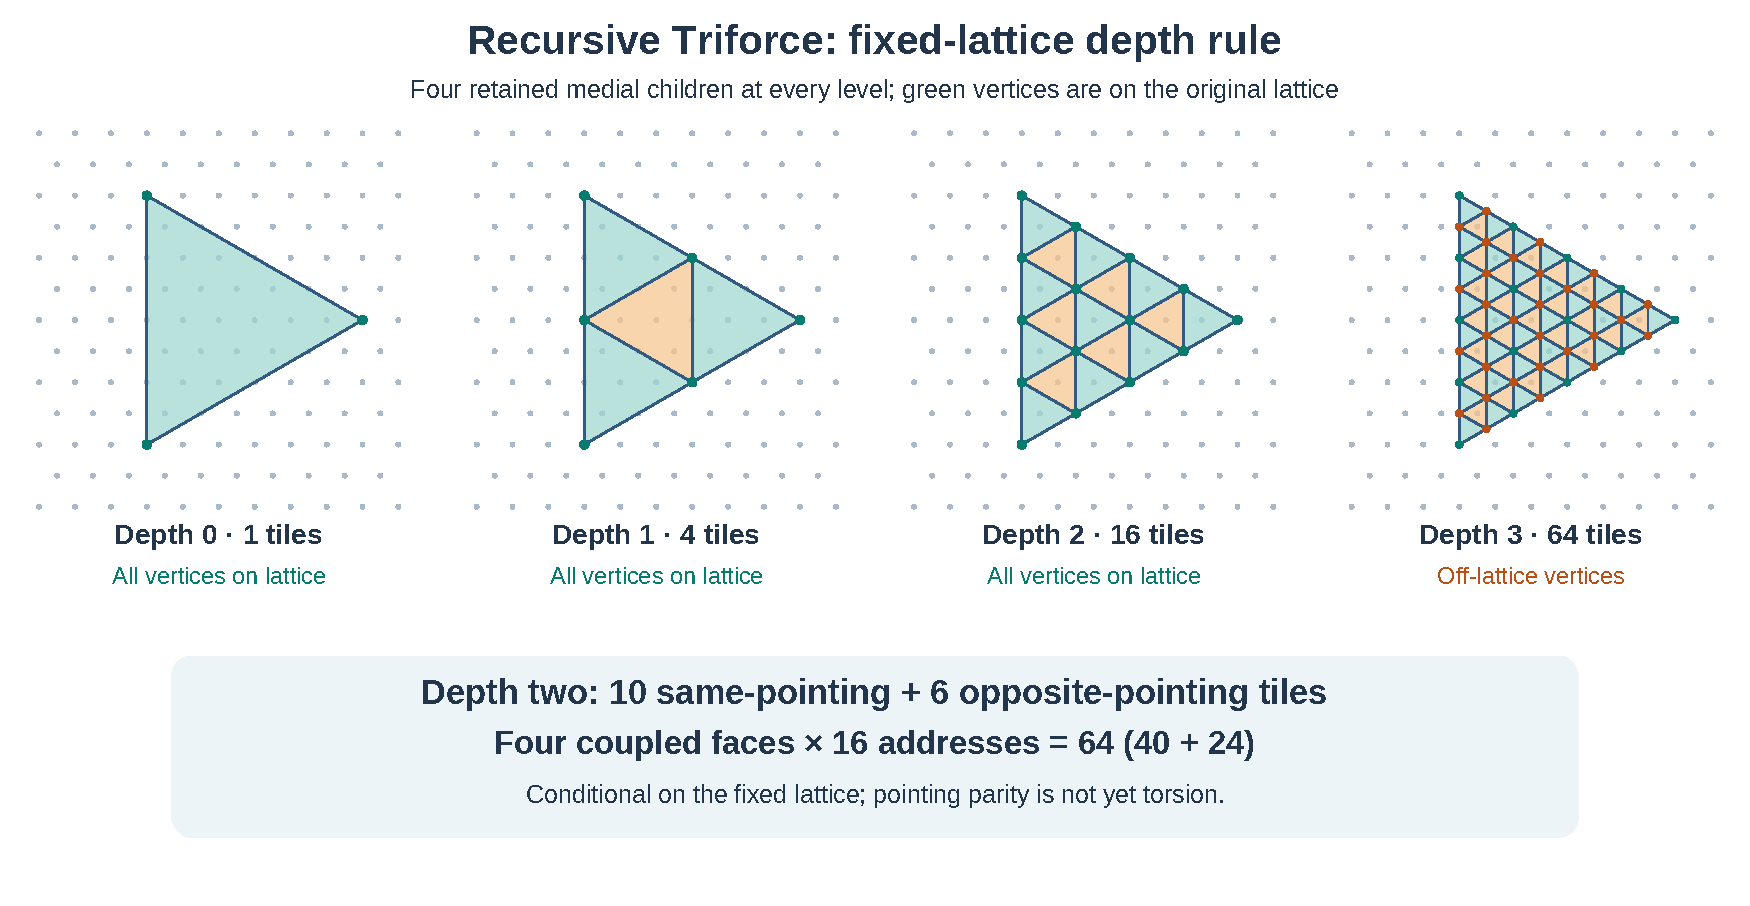
\includegraphics[width=\columnwidth]{recursive_triforce_figure.pdf}
\caption{The fixed midpoint lattice permits two full dyadic refinements; the third contains off-lattice vertices. Green and orange distinguish pointing, not chirality.}
\end{figure}
\begin{figure}[!t]
\centering
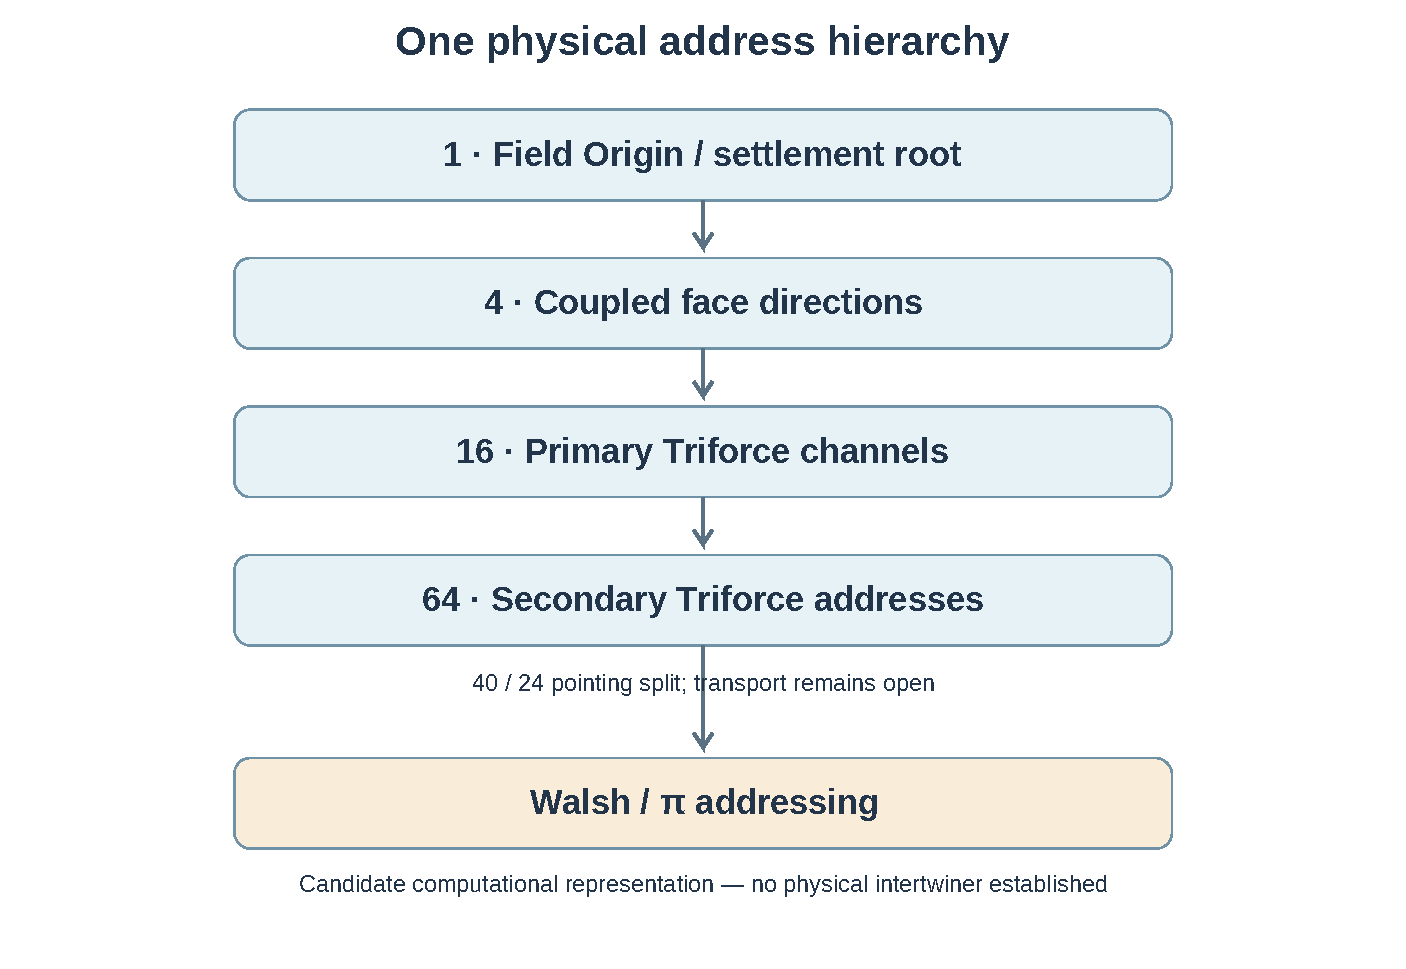
\includegraphics[width=\columnwidth]{closure_hierarchy_figure.pdf}
\caption{One paired geometric hierarchy. The Walsh and $\pi$ operations remain candidate representations or addressing mechanisms.}
\end{figure}
\end{document}
